\chapterimage{capitulo01.jpg} % Chapter heading image
\chapter{ Introdução}
  % Prof. Dr. Ausberto S. Castro Vera
  % UENF - CCT - LCMAT - Curso de Ciência da Computação
  % Campos, RJ,  2021
  % Disciplina: Paradigmas de Linguagens de Programação
  % Aluno: João Vítor Fernandes Dias
  Este documento apresentará os aspectos gerais da linguagem de programação denominada R. Passaremos brevemente sobre os diversos tópicos relacionados às capacidades da linguagem, tais como sua história, estrutura de código, seus paradigmas de linguagem, dentre outros.

  Agora nos limitando a este capítulo, iremos aprender sobre os momentos importantes da história da linguagem R e também sobre as áreas onde a linguagem é mais utilizada.

  \section{Aspectos históricos da linguagem R}

    R é uma linguagem e ambiente para computação estatística e gráfica \cite{Eglen2009}. Ele é similar à linguagem S, portanto, boa parte dos códigos S são compreendidos no mesmo ambiente do R. Ele foi desenvolvido e é mantido pelo núcleo de programadores (R-core). Essa linguagem tem seu nome devido ao nome de seus criadores Ross Ihaka e Robert Gentleman e também por causa do nome da linguagem S da qual foi baseada.
    %https://en.wikipedia.org/wiki/R_(programming_language)

    R passou a ser utilizado amplamente em diversas áreas da computação científica por sua capacidade de visualização estatística (como pode ser visto na Fig.\ref{R_Graphs}). Além disso, por ser um software gratuito, não há ônus para os pesquisadores ao utilizá-lo em suas pesquisas.

    \begin{comment}
      https://rkabacoff.github.io/datavis/datavis.pdf
      https://web.stanford.edu/class/bios221/book/Chap-Graphics.html
      https://www.r-graph-gallery.com/index.html
      https://www.r-project.org/
    \end{comment}
    \begin{figure}[H]
      \begin{center}
        \caption{Gráficos feito com a linguagem R} \label{R_Graphs}
        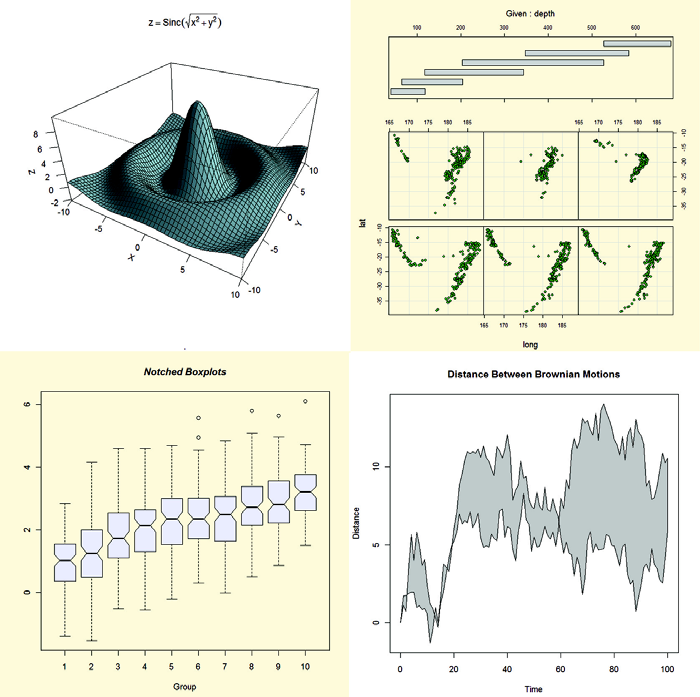
\includegraphics[width=12cm]{R_in_action_Graphs.png} \\
        {\tiny \sf Fonte: \cite{Kabacoff2015}}
      \end{center}
    \end{figure}

    A utilização da linguagem R está associado ao uso de pacotes (packages, em inglês) o que auxilia no rápido acesso e instalação do software o que facilita a utilização pela comunidade científica.\cite{Chambers2014}

    Dos diversos paradigmas de programação existentes, a linguagem R utiliza de duas delas: programação funcional e programação orientada a objetos (POO) que será abordada futuramente neste documento.\cite{Chambers2014}


  \section{áreas de Aplicação da Linguagem}
    Diversas áreas são contempladas com o uso da linguagem R. Dentre elas podemos citar as seguintes:

    \subsection{ Data Science}
      Para utilizarmos o potencial que o R tem em relação a ciência de dados, primeiro precisamos entender a sequência necessária para o trabalho com os dados descritor por \cite{HadleyWickham2017} e ilustrados em \ref{R_data_cycle}:

      \begin{enumerate}
        \item \textbf{Importar para o R}
          Não dá para utilizarmos os dados sem tê-los em mãos.
        \item \textbf{Wrangling}
          Essa etapa engloba o tratamento de dados. Ela se refere ao processo onde os dados são limpos e transformados. O termo em inglês "wrangling" significa "luta" porque você está "lutando" contra a bagunça dos dados.
        \begin{enumerate}
          \item \textit{Limpar}
            Com "limpar" quero dizer "guardar os dados de forma ordenada". Em dados organizados em planilhas, por exemplo, cada coluna representa uma variável e cada linha representa um de seus valores.
            Organizá-la ajuda a poder trabalhar com ela de forma mais consistente.
          \item \textit{Transformar}
            Nessa etapa você precisará filtrar o que de fato é relevante dentro dos dados que se tem, removendo o que não convém e se necessário, utilizando dos dados iniciais para calcular novas colunas de dados.
        \end{enumerate}
        \item \textbf{Processo de geração de conhecimento}
          É o modo como você irá analisar e obter conhecimento a partir dos dados. Existem dois meios principais, a visualização e a modelagem. Cada um deles tem suas vantagens e desvantagens, por isso numa análise real, será necessário alternar entre eles.
        \begin{enumerate}

          \item \textit{Visualização}

            É fundamentalmente uma tarefa humana. Com uma boa visualização e análise, consegue-se obter boas informações, algumas vezes até inesperadas. Isso pode levantar novas questões ou indicar que não se está analisando os dados certos para o problema abordado. Entretanto, o fato de depender da análise humana, impede uma boa escalabilidade.
          \item \textit{Modelos}
            É fundamentalmente computacional e matemático. Um modelo bem feito é utilizado para se obter respostas diretas e precisas em relação aos dados analisados pelo modelo, entretanto, um modelo não é capaz de se questionar quando a ele próprio, pois são os programadores que definem seus parâmetros. Caso algo não tenha sido desenvolvido apropriadamente, os resultados podem não ser satisfatórios. Entretanto, o fato de depender da análise computacional e matemática, permite uma boa escalabilidade.
        \end{enumerate}
      %          \item \textbf{4. Comunicação}
      %################################
      %Preencher a parte de comunicação
      %################################

      \end{enumerate}

      \begin{figure}[H]
        \begin{center}
          \caption{Fluxo dos dado} \label{R_data_cycle}
          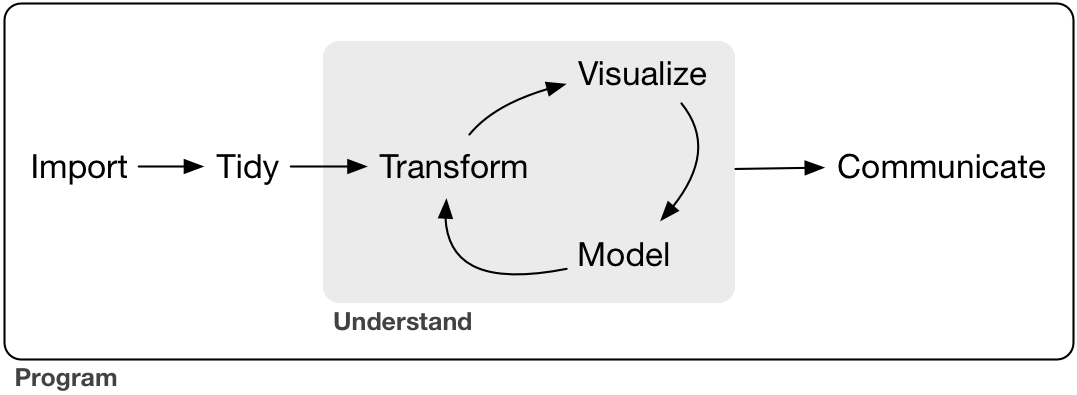
\includegraphics[width=12cm]{R_for_data_science_data_cycle.png} \\
          {\tiny \sf Fonte: \cite{HadleyWickham2017} }
        \end{center}
      \end{figure}

    \subsection{ Paradigmas}

      Como dito por \cite{Chambers2014} As evoluções na linguagem a levaram a ter suas próprias versões de programação funcional e orientada a objetos. O objetivo da evolução não foi o design em si, mas sim prover as ferramentas necessárias para pesquisa e análise de dados pela comunidade na época.Ela começou com a reprodução de funcionalidades da linguagem S, onde eram utilizados bibliotecas estatísticas, principalmente em Fortran.

      \begin{comment}
        In the case of functional programming, the realization in R is only partial, reflecting the language’s origins as well as practical considerations. In the case of OOP, there are now at least three realizations of the ideas in R, using two different paradigms. All three have significant applications and practical value. Despite all these devilish details, the main ideas remain visible and useful, particularly when programming serious applications using the language.
      \end{comment}

      Para entender essas questões computacionais em R, dois slogans podem ajudar:
      \begin{itemize}
        \item Tudo que existe é um objeto.
        \item Tudo que acontece é a chamada de uma função.
      \end{itemize}

      \subsubsection{ Orientação a objetos}

        Segundo \cite{Chambers2014} os ideis de POO em R são bem simples e intuitivas:
        \begin{enumerate}
          \item Tudo que utilizamos é um objeto e objetos devem ser estruturados para cumprir os objetivos do nosso uso.
          \item Para isso utilizaremos das relações entre diversas classes e objetos contendo atributos que interagem entre si.
          \item Uma classe pode herdar (conter) uma superclasse. Assim, seu objeto também será um objeto da superclasse.
          \item Para trabalharmos com objetos, podemos definir métodos para certas classes.
        \end{enumerate}

        Afinal, R é uma linguagem orientada a objetos? Não completamente, mas dispõe de softwares que refletem os mesmos conceitos.
        Porém, por ser uma linguagem principalmente funcional, acaba permitindo que suas definições de classe e objeto sejam feitas de diversas formas diferentes, isto faz com que acabe havendo certa confusão quanto a isso.

        Por exemplo: em R, os métodos pertencem às funções e não aos objetos em si. Por causa dessa e outras especificidades da linguagem, podemos chamá-la de uma linguagem funcional orientada a objetos, já que para ser verdadeiramente orientada a objetos, seus métodos precisariam estar encapsulados nos objetos.

        \begin{comment}
          Some of the confusion arises from not recognizing that the final item in the list above can be implemented in radically different ways, depending on the
          general paradigm of the programming language. A
          key distinction is whether the methods are to be
          embedded in some form of functional programming.
          Traditionally, most languages adopting the OOP
          %paradigm are not functional; either the language be-
          gan with objects and classes as a central motivation
          (SIMULA, Java) or added the paradigm to an exist-
          ing non-functional language (C++, Python). In such
          languages, methods were naturally associated with
          classes, essentially as callable properties of the ob-
          jects. The language would then include syntax to
          call or invoke a method on a particular object, most
          often using the infix operator “.”. The class defini-
          tion then encapsulates all the software for the class.
          Where methods are needed for other computations,
          such as special method names in Python or opera-
          tor overloading in C++, these are provided by ad-
          hoc mechanisms in the language, but the method
          remains part of the class definition.
          In a language that is functional or that aspires to
          behave functionally as S and R do, the natural role
          of methods corresponds to the intuitive meaning of
          “method”—a technique for computing the desired
          result of a function call. In functional OOP, the par-
          ticular computational technique is chosen because
          one or more arguments are objects from recognized
          classes.
          Methods in this situation belong to functions, not
          to classes; the functions are generic. In the simplest
          and most common case, referred to as a standard
          generic function in R, the function defines the formal
          arguments but otherwise consists of nothing but a
          table of the corresponding methods plus a command
          to select the method in the table that matches the
          classes of the arguments. The selected method is a
          function; the call to the generic is then evaluated as
          a call to the selected method.
          We will refer to this form of object-oriented pro-
          gramming as functional OOP as opposed to the encapsulated
          form in which methods are part of the
          class definition.
        \end{comment}

      \subsubsection{ Programação Funcional}
        Seguindo as ideias propostas por \cite{Chambers2014} a programação funcional tem princípios que nos ajudam no desenvolvimento confiável de funções para diferentes modelos, já a POO auxilia com as ferramentas necessárias para se definir o modelo devidamente.

        Veremos agora alguns princípios da programação funcional resumidamente:

        \begin{enumerate}
          \item A programação depende amplamente da definição de funções
          \item Uma função retorna um valor único de acordo com os valores passados a ela.
          \item A chamada de uma função não causa efeitos colaterais em outros cálculos.
        \end{enumerate}

        Linguagens verdadeiramente funcionais se conformam a estas ideias, tanto pelo que dispõem quanto pelo que não dispõem. Nesse sentido, R é uma linguagem funcional? Não. A sua estrutura não reforça a funcionalidade. Sua estrutura poderia ser reescrita para comportar plenamente a funcionalidade, mas isso precisaria modificar também algumas questões da linguagem que já foram bem analisadas, como por exemplo a geração de números aleatórios que é baseado no uso de estados.

        Apesar de suas limitações, a linguagem funcional permanece sendo de extrema importância para a programação estatística, como pode ser exemplificado pelos modelos estatísticos de dados frequentemente desenvolvidos em R e analisados através de uma perspectiva funcional.

        \begin{comment}
          Is R a functional programming language in this
          sense? No. The structure of the language does
          not enforce functionality; Section 2.3 examines that
          structure as it relates to functional programming
          and OOP. The evolution of R from earlier work in
          statistical computing also inevitably left portions of
          earlier pre-functional computations; Section 3 out-
          lines the history. Random number generation, for ex-
          ample, is implemented in a distinctly “state-based”
          model in which an object in the global environ-
          ment (.Random.seed) represents the current state
          of the generators. Purely functional languages have
          developed techniques for many of these computa-
          tions, but rewriting R to eliminate its huge body of
          supporting software is not a practical prospect and
          would require replacing some very well-tested and
          well-analyzed computations (random number gen-
          eration being a good example).
          Functional programming remains an important

          paradigm for statistical computing in spite of these
          limitations. Statistical models for data, the motivat-
          ing example for many features in S and R, illustrate
          the value of analyzing the software from a functional
          programming perspective. Software for fitting mod-
          els to data remains one of the most active uses of
          R. The functional validity of such software is im-
          portant both for theoretical justification and to de-
          fend the results in areas of controversy: Can we show
          that the fitted models are well-defined functions of
          the data, perhaps with other inputs to the model
          such as prior distributions considered as additional
          arguments? The structure of R as described in Sec-
          tion 2.3 can provide support for analyzing functional
          validity. Equally usefully, such analysis can also illu-
          minate the limits of functional validity for particular
          software, such as that for model-fitting.
        \end{comment}